\chapter{Reporte de Defectos}
\label{apendice:c}

\section{Detalle de Defectos}

\begin{longtable}{lccccp{5cm}}
\caption{Reporte detallado de defectos}
\label{tab:reporte-defectos}\\
\toprule
\textbf{ID} & \textbf{RF} & \textbf{Severidad} & \textbf{Prioridad} & \textbf{Estado} & \textbf{Descripción}\\
\midrule
\endfirsthead
\toprule
\textbf{ID} & \textbf{RF} & \textbf{Severidad} & \textbf{Prioridad} & \textbf{Estado} & \textbf{Descripción}\\
\midrule
\endhead
\bottomrule
\endfoot

BUG-002 & RF-03 & Minor & Low & Abierto & Error ``No se encontró la referencia'' en consola al detener la grabación. No impide la funcionalidad.\\

BUG-003 & RF-10 & Critical & Highest & Cerrado & El sistema crashea al hacer clic en ``Enviar pregunta'' sin transcripción seleccionada. Corregido en commit 7e61c36.\\

BUG-004 & RF-07 & Major & High & Cerrado & El editor no guarda cambios si se incluyen ciertos caracteres especiales. Corregido en commit a1b2c3d.\\

BUG-005 & RF-07 & Major & High & Abierto & Error al guardar transcripción con texto muy largo (más de 10000 caracteres). En investigación.\\

BUG-006 & RF-01 & Minor & Low & Abierto & Tooltip duplicado en el botón de logout. No impide la funcionalidad.\\

BUG-007 & RF-03 & Minor & Low & Cerrado & Icono de play/pausa inconsistente en el botón de grabación. Corregido en commit e4f5g6h.\\

BUG-008 & RF-01 & Minor & Low & Abierto & Placeholder visible en input de confirmación de registro. No impide la funcionalidad.\\

BUG-009 & RF-05 & Minor & Low & Abierto & Texto de ayuda ``Eliminar completamente esta nota de voz'' visible en upload. No impide la funcionalidad.\\

\bottomrule
\end{longtable}

\section{Distribución por Severidad}

\begin{itemize}
    \item \textbf{Critical:} 1 (BUG-003) -- Corregido
    \item \textbf{Major:} 2 (BUG-004, BUG-005) -- 1 corregido, 1 abierto
    \item \textbf{Minor:} 5 (BUG-002, BUG-006, BUG-007, BUG-008, BUG-009) -- 1 corregido, 4 abiertos
\end{itemize}

\section{Evidencias de Casos Fallidos en Flujos Críticos}

Las siguientes evidencias corresponden a ejecuciones manuales registradas en Zephyr. Se presentan por caso de prueba y requisito, sin asignar identificadores de ticket que no son visibles en las capturas. CP-09 fue corregido y aprobado en re-prueba; CP-05 y CP-16 permanecen pendientes.

\begin{longtable}{p{1.5cm}p{1.5cm}p{7.2cm}>{\RaggedRight\arraybackslash}p{3.4cm}}
\caption{Incidencias observadas en casos de flujos críticos}
\label{tab:evidencias-fallos-criticos}\\
\toprule
\textbf{Caso} & \textbf{RF} & \textbf{Hallazgo observado} & \textbf{Estado al cierre}\\
\midrule
\endfirsthead
\toprule
\textbf{Caso} & \textbf{RF} & \textbf{Hallazgo observado} & \textbf{Estado al cierre}\\
\midrule
\endhead
\bottomrule
\endfoot
CP-05 & RF-05 & El procesamiento del audio inicia, pero al finalizar no se crea ni aparece la nota transcrita en el listado. & \textcolor{FalloColor}{Abierto}\\
CP-09 & RF-09 & El job de formateo inicia, pero el contenido del editor no se actualiza con la respuesta de IA. & \textcolor{PasoColor}{Corregido y re-probado}\\
CP-16 & RF-05 & La interfaz acepta la selección de un archivo no admitido en vez de rechazarlo antes del envío. & \textcolor{FalloColor}{Abierto}\\
\bottomrule
\end{longtable}

\subsection{CP-05: transcripción no generada}

La ejecución supera la selección del archivo y el inicio del procesamiento. El fallo se presenta en el paso 6: una vez concluido el proceso, la transcripción esperada no aparece en el listado. La evidencia de la Figura~\ref{fig:evidencia-critica-cp05} muestra el paso previo aprobado y el resultado final fallido.

\begin{figure}[H]
\centering
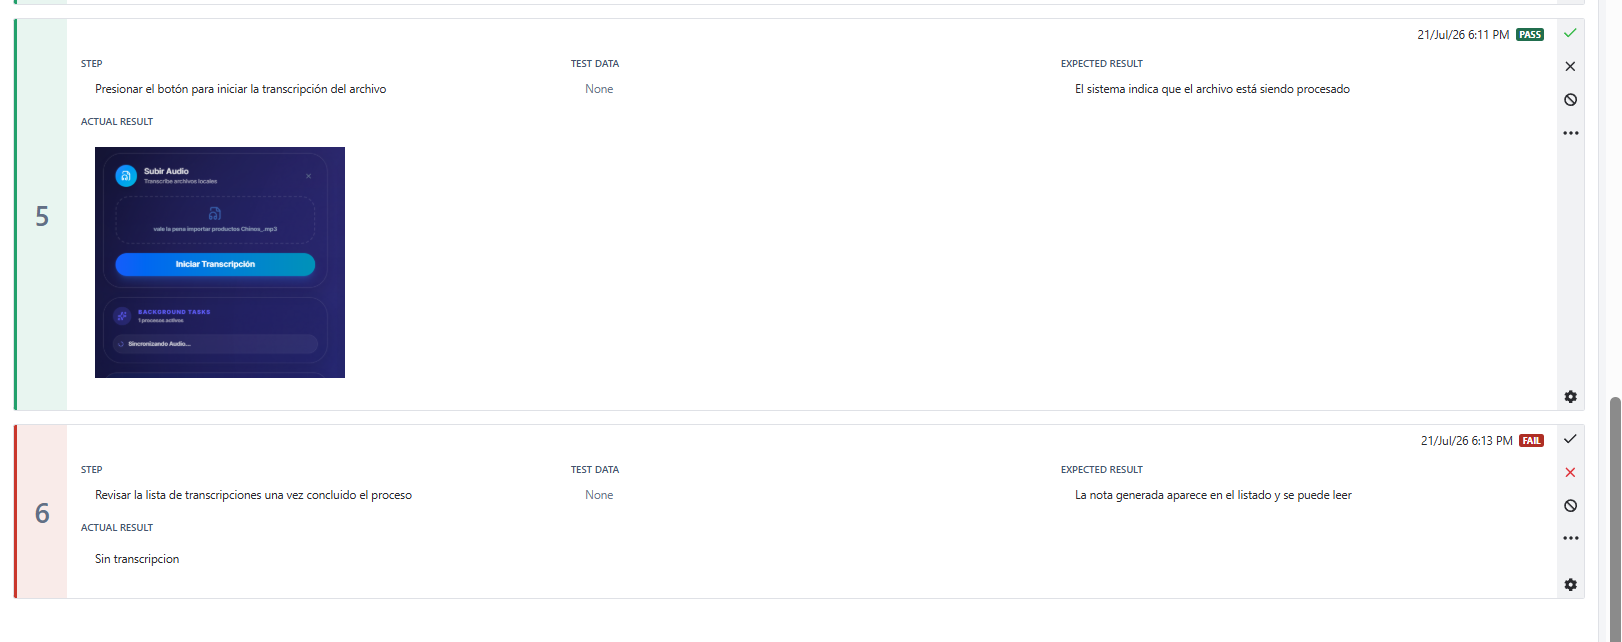
\includegraphics[width=\textwidth]{../../informe/images/caso-critico1.png}
\caption{CP-05: procesamiento iniciado sin generación posterior de la transcripción}
\label{fig:evidencia-critica-cp05}
\end{figure}

\subsection{CP-09: formateo IA sin actualización del editor}

La primera ejecución confirmó que el backend aceptaba la solicitud y creaba el job, pero el paso 5 falló porque el visor no recibía el texto formateado. Después de levantar la incidencia se identificaron dos causas técnicas: el WebSocket intentaba publicar un objeto de progreso fuera del flujo válido y la integración dependía de un modelo no habilitado para la cuenta, lo que producía una respuesta 404 del proveedor.

La solución consistió en transmitir dentro del ciclo asíncrono cada actualización entregada por el agente de formateo, seleccionar un modelo NVIDIA NIM disponible con alternativas de respaldo y guardar el contenido formateado en la transcripción. Se añadió cobertura de regresión para el progreso WebSocket y la finalización del job. En la re-prueba, el evento de finalización llegó al frontend y el editor mostró el contenido actualizado.

\begin{figure}[H]
\centering
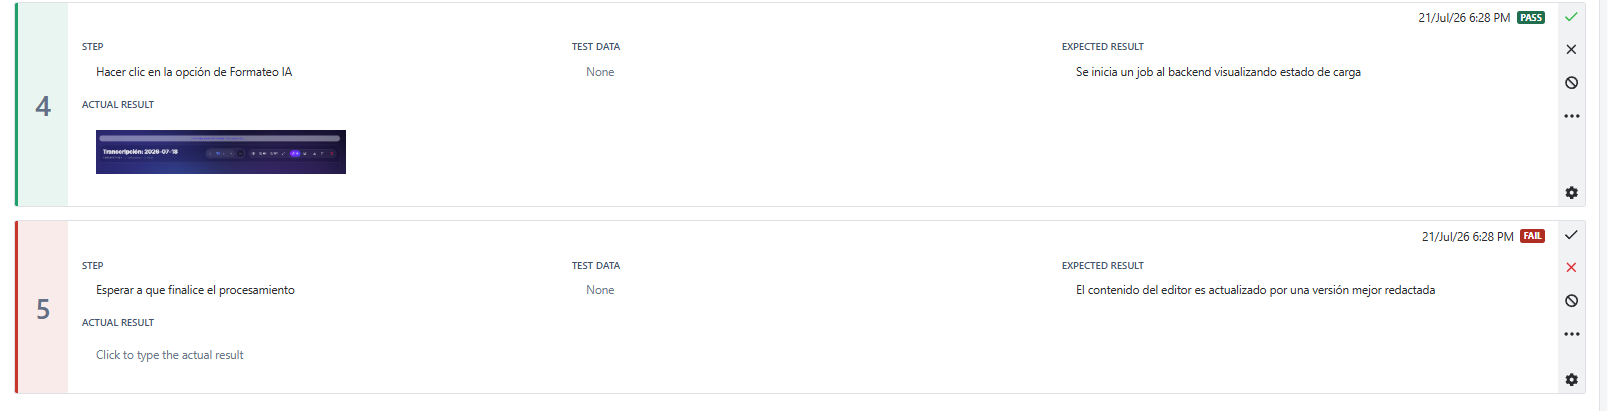
\includegraphics[width=\textwidth]{../../informe/images/caso-critico2.png}
\caption{CP-09: evidencia de la ejecución inicial fallida antes de la corrección}
\label{fig:evidencia-critica-cp09}
\end{figure}

\clearpage
\subsection{CP-16: archivo de formato inválido aceptado}

El selector debía impedir la carga de archivos \texttt{.txt} o \texttt{.pdf} antes de contactar al backend. La ejecución evidenció que la interfaz permitió seleccionar un archivo no admitido, por lo que la validación local no cumplió el resultado esperado. La incidencia continúa abierta.

\begin{figure}[H]
\centering
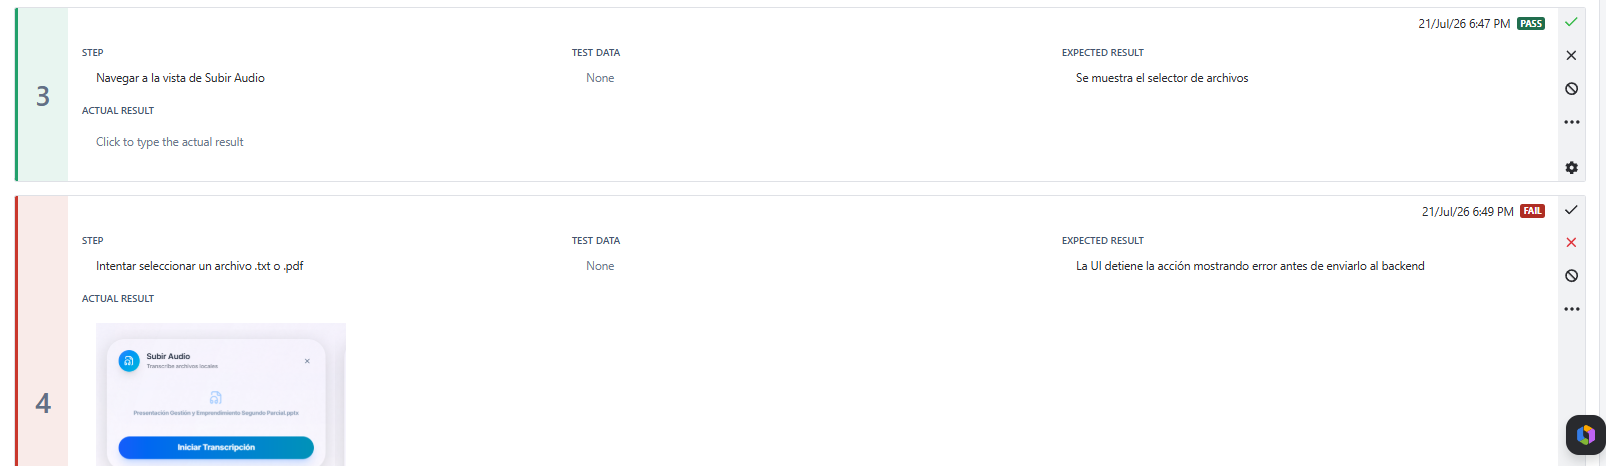
\includegraphics[width=\textwidth]{../../informe/images/caso-critico3.png}
\caption{CP-16: selección permitida de un formato no admitido por la interfaz}
\label{fig:evidencia-critica-cp16}
\end{figure}
